%%%%%%%%%%%% 选择学位类型:专硕%%%%%%%%%%
\documentclass[EnMaster]{BJTU-thesis}  %%专硕
\usepackage[T1]{fontenc}  %设置英文字体为times new roman
\usepackage{mathptmx}
 

%%%%%%%%%%%%%%%%%填写封面信息%%%%%%%%%%%%%%%%%%%%%%%%
\author{张三}                                  %作者姓名
\studentNumber{11111111}                       %作者学号
\advisor{李四}                                 %导师姓名
\advisorTitle{教授}                            %导师职称
\degreeType{工学}                              %学位类别
\major{计算机科学技术}                         %所属专业
\researchArea{模式识别}                        %研究方向
\title{论文题目}                               %论文题目
\englishtitle{The Title in English.}           %论文题目英文
\datetime{2019年6月}                           %编辑日期


%%%%%%%%%%%%%%%%%%%%%%%%%%%%%%%%%%%%%%%%%%%%%%
%\setmainfont{Times New Roman}

\begin{document}
	\makecover
	\makeAuthorization
	\makeInfo
	 \setlength{\baselineskip}{20pt}
\begin{thanks}
[内容为小四号宋体。]放置在摘要页前,对象包括:1)国家科学基金,资助研究工作的奖学金基金,合同单位,资助或支持的企业、组织或个人。2)协助完成研究工作和提供便利条件的组织或个人。3)在研究工作中提出建议和提供帮助的人。4)给予转载和引用权的资料、图片、文献、研究思想和设想的所有者。5)其他应感谢的组织和个人。


\end{thanks} 									 %致谢部分
	\setlength{\baselineskip}{20pt}
\begin{abstract}
	[内容为小四号宋体。] 中文摘要应将学位论文的内容要点简短明了地表达出来,硕士学位论文一般为500~1000字,博士学位论文一般为1000~2000字。留学生英文版学位论文不少于3000字中文摘要,留学生英文版博士学位论文不少于5000字中文摘要。字体为宋体小四号。内容应包括工作目的、研究方法、成果和结论。要突出本论文的创新点,语言力求精炼。为了便于文献检索,应在本页下方另起一行注明论文的关键词(3-8个),如有可能,尽量采用《汉语主题词表》等词表提供的规范词。图X幅,表X个,参考文献X篇。

		
	\noindent\keywords{[请输入关键词(3-8),以分号分隔。] }
\end{abstract}   								 %中文摘要
	 \setlength{\baselineskip}{20pt}
\begin{englishabstract}
	"[内容为小四号Times New Roman。]" 一般为1000个左右实词。
	
	\noindent\englishkeywords{[请输入英文关键词,与中文关键词保持一致。以分号分隔。] }
\end{englishabstract}  							 %英文摘要
      \setlength{\baselineskip}{20pt}
\begin{preface}
	[鼠标左键单击选择该段落,输入替换之。内容为小四号宋体。] 学位论文的序或前言,一般是作者或他人对本篇论文基本特征的简介,如说明研究工作缘起、背景、主旨、目的、意义、编写体例,以及资助、支持、协作经过等;也可以评述和对相关问题发表意见。这些内容也可以在正文引言中说明。
		
	
\end{preface}                                             %序言

	
	
	\tableofcontents
     \newpage\pagenumbering{arabic}

     %正文部分
      \setlength{\baselineskip}{20pt}
\chapter{引言}
\label{cha:intro}

[鼠标左键单击选择该段落,输入替换之。内容为小四号宋体。] 引言(或绪论)简要说明研究工作的目的、范围、相关领域的前人工作和知识空白、理论基础和分析、研究设想、研究方法和实验设计、预期结果和意义等。应言简意赅,不要与摘要雷同,不要成为摘要的注释。一般教科书中有的知识,在引言中不必赘述。




 								%引言
      \setlength{\baselineskip}{20pt}
\chapter{1级标题}
\label{cha:chap2}

[鼠标左键单击选择该段落,输入替换之。内容为小四号宋体。] 学位论文为了需要反映出作者确已掌握了坚实的基础理论和系统的专门知识,具有开阔的科学视野,对研究方案作了充分论证,因此,有关历史回顾和前人工作的综合评述,以及理论分析等,可以单独成章,用足够的文字叙述。正文是学位论文的核心部分,占主要篇幅,可以包括:调查对象、实验和观测方法、仪器设备、材料原料、实验和观测结果、计算方法和编程原理、数据资料、经过加工整理的图表、形成的论点和导出的结论等。


由于研究工作涉及的学科、选题、研究方法、工作进程、结果表达方式等有很大的差异,对正文内容不能作统一的规定。但是,必须实事求是,客观真切,准确完备,合乎逻辑,层次分明,简练可读。


\textbf{图}:见《北京交通大学学位论文撰写规范》3.10.4
\begin{figure}[!htb] % use float package if you want it here
	%\setlength{\abovecaptionskip}{-0.2cm} %调整图片caption与正文之间的间距,table同理。可自己调整。
	\setlength{\belowcaptionskip}{-0.2cm} 
	\centering
	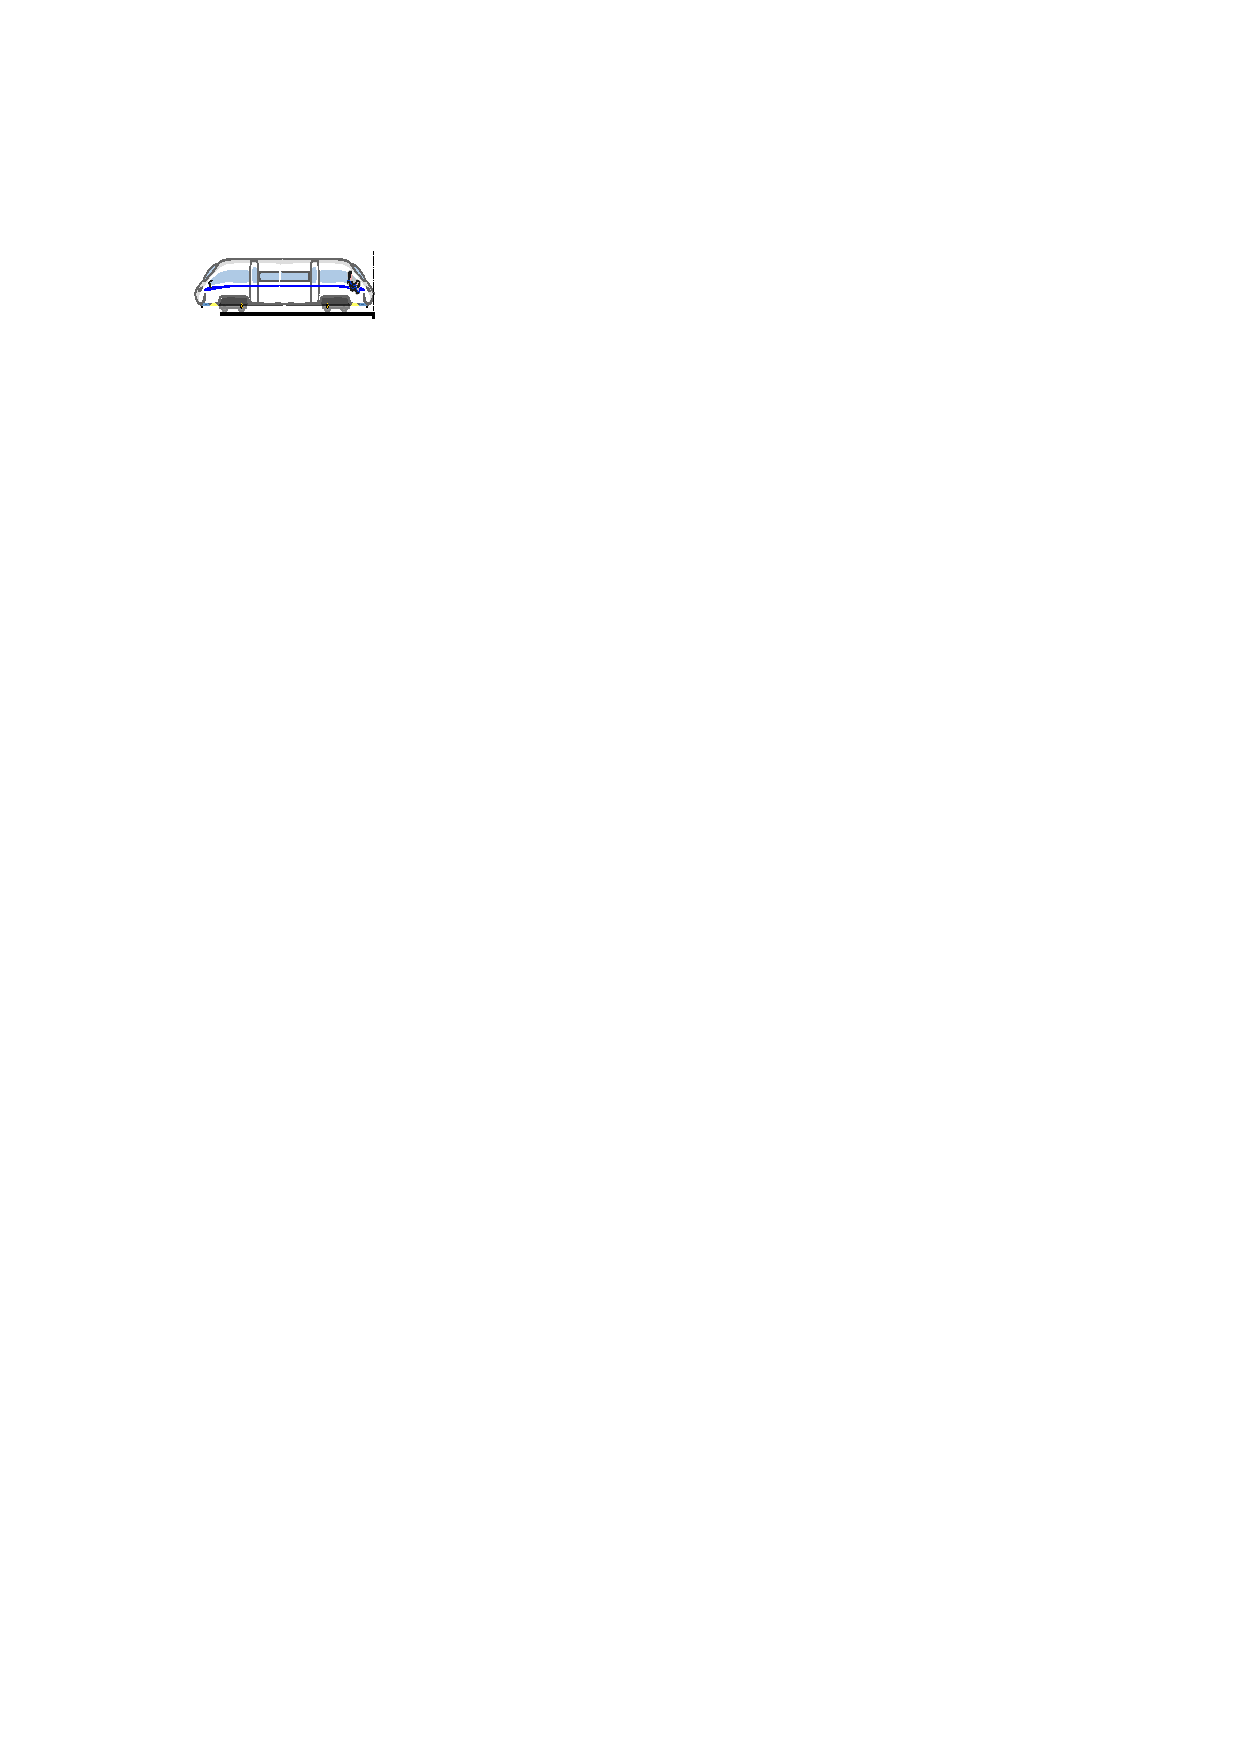
\includegraphics[scale=1]{figures/figure1.pdf}
	\caption{示例图片。\\Fig~\ref{fig:02:01}~Example of Figure.}
	\label{fig:02:01}
\end{figure}

图应有编号。图的编号由“图”和从“1”开始的阿拉伯数字组成,图较多时,可分章依序编号。

图宜有图题,图题即图的名称,置于图的编号之后。图的编号和图题应置于图下方。图题采用中英文对照,英文(Times New Roman)字体五号,中文宋体五号。居中书写,中文在上。

照片图要求主题和主要显示部分的轮廓鲜明,便于制版。如用放大缩小的复制品,必须清晰,反差适中。照片上应有表示目的物尺寸的标度。

例如:如图\ref{fig:02:01}所示
\begin{figure}[h]
	%\setlength{\abovecaptionskip}{-0.2cm} %调整图片caption与正文之间的间距,table同理。可自己调整。
	\setlength{\belowcaptionskip}{-0.2cm} 
	\centering
	\addtocounter{subfigure}{-1}\subfigure[English caption1] {\subfigure[中文标题1] { 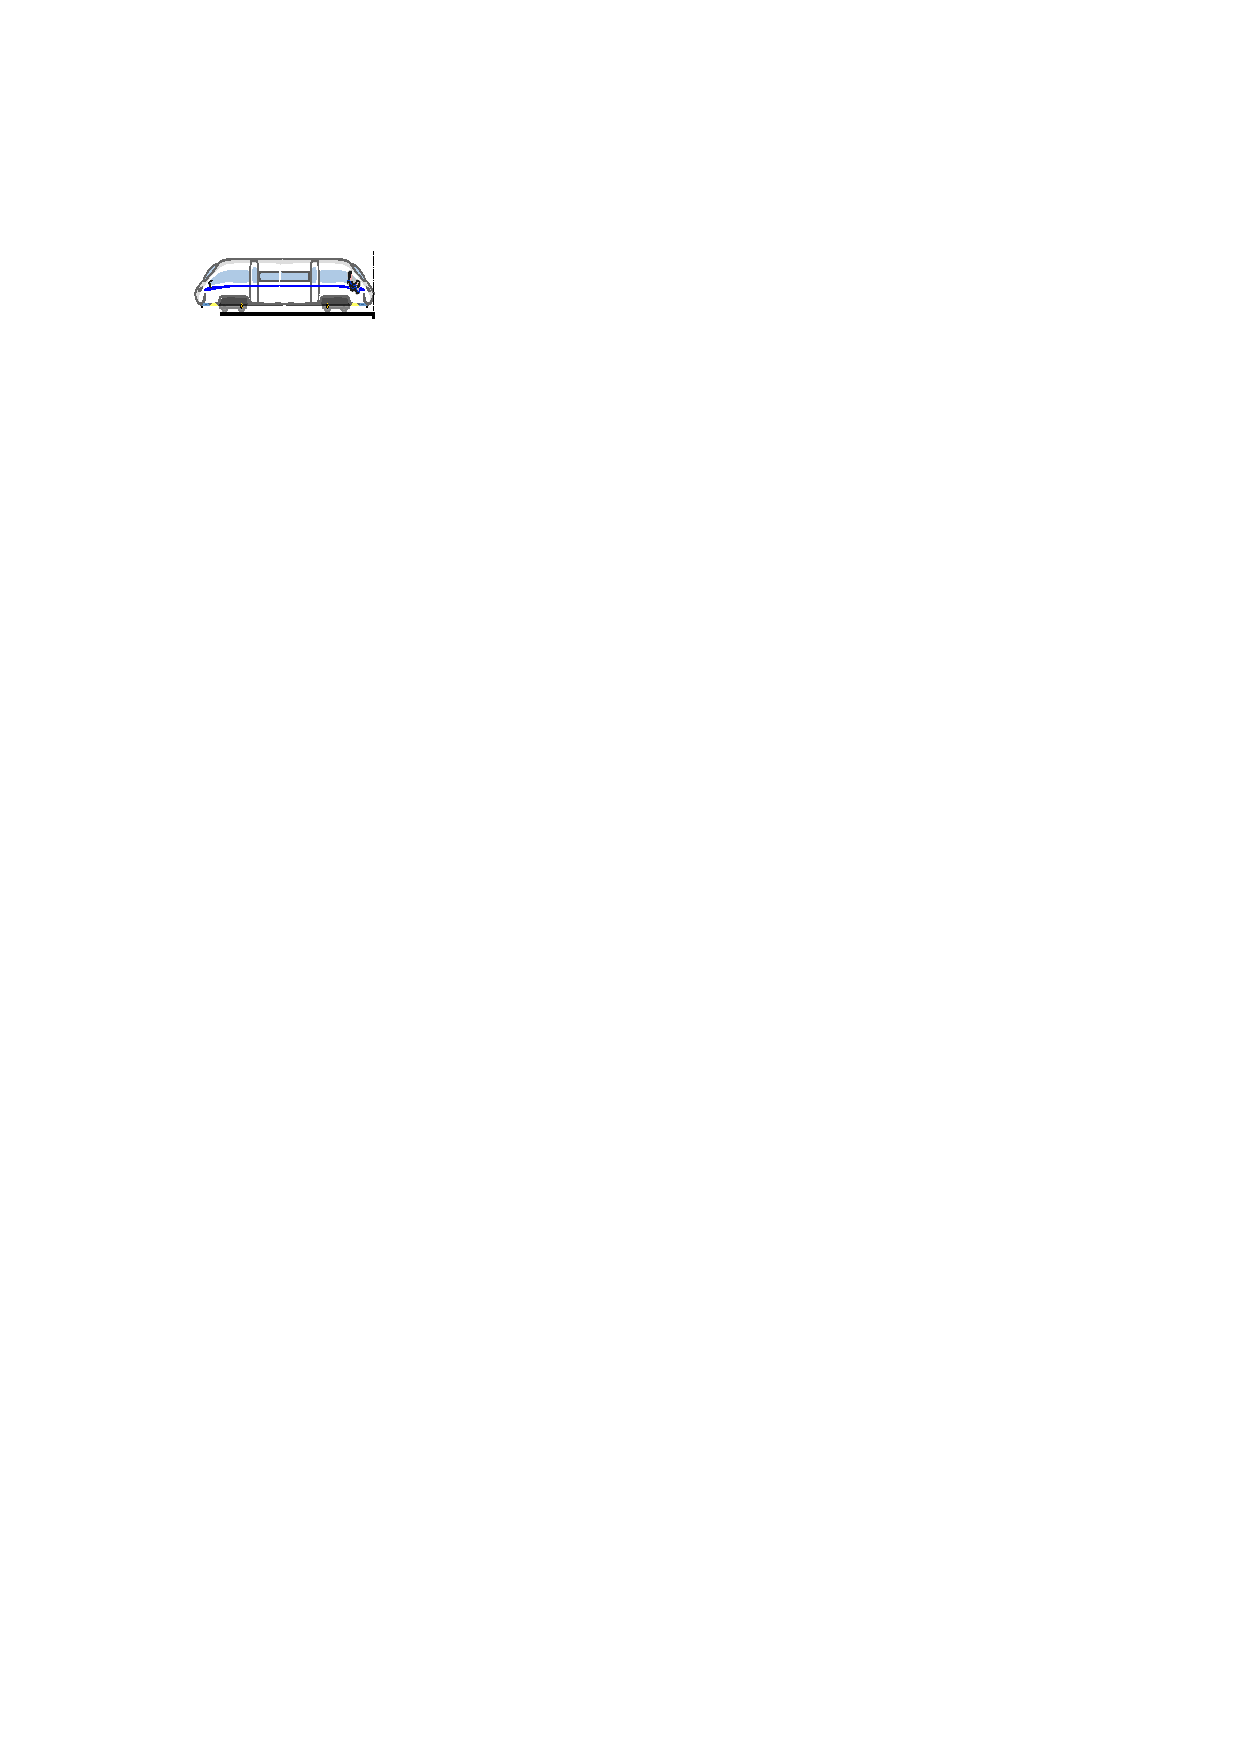
\includegraphics[scale=1]{figures/figure1.pdf}}}
	\addtocounter{subfigure}{-1}\subfigure[English caption2] {\subfigure[中文标题2]{ 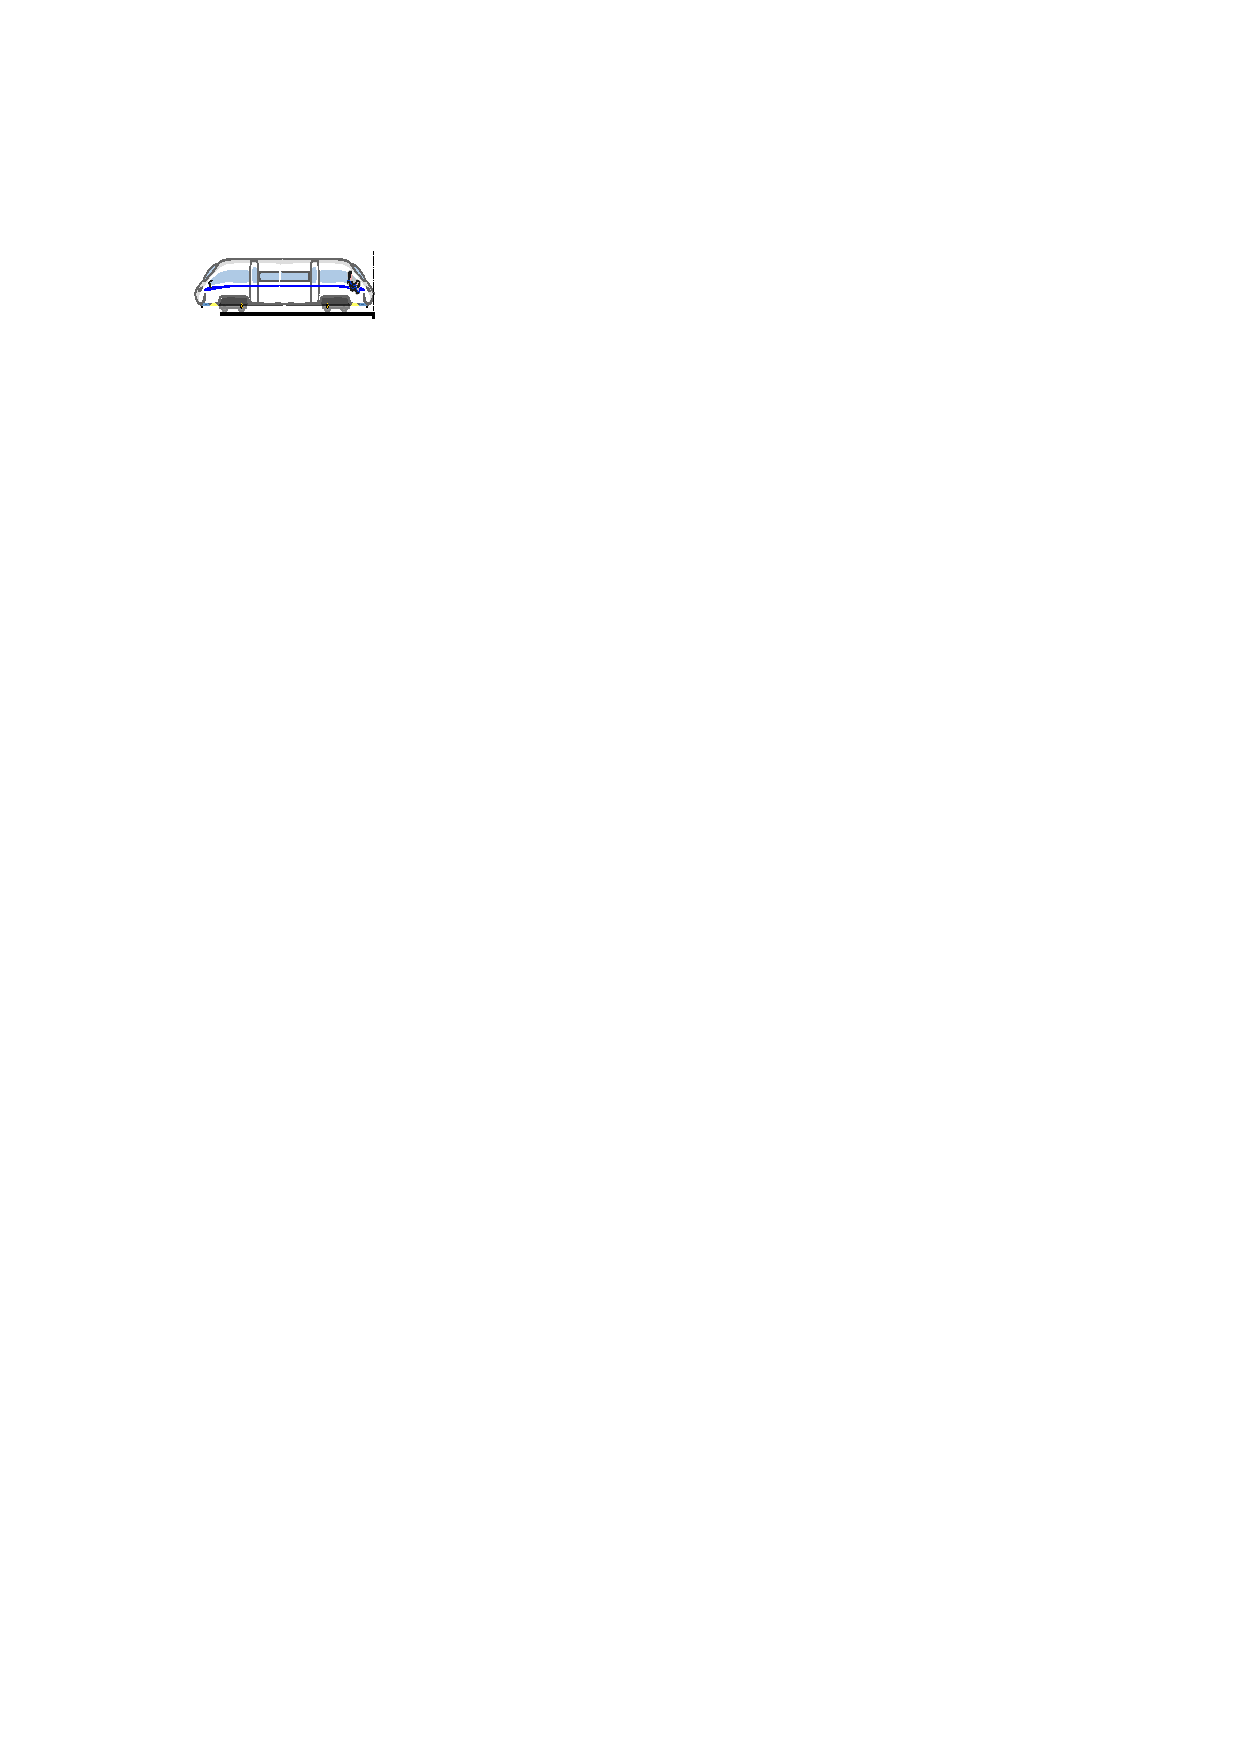
\includegraphics[scale=1]{figures/figure1.pdf}}}
	\caption{示例图片。\\Fig~\ref{fig:02:02}~Example of Figure.}
	\label{fig:02:02}
\end{figure} 

\textbf{表}:见《北京交通大学学位论文撰写规范》3.10.5

表应有编号。表的编号由“表”和从“1”开始的阿拉伯数字组成,表较多时,可分章依序编号。

表宜有表题,表题即表的名称,置于表的编号之后。表的编号和表题应置于表上方。表题采用中英文对照,居中,中文在上。英文(Times New Roman)字体五号,中文宋体五号。

表的编排,一般是内容和测试项目由左至右横读,数据依序竖读。
表的编排建议采用国际通行的三线表。

如某个表需要转页接排,在随后的各页上应重复表的编号。编号后跟表题(可省略)和“(续)”,置于表上方。
续表均应重复表头。

例如:如表格\ref{table:02:01}所示

\begin{table}[!htb]\small   %%\small是为了设置表格中的字体比正文小
	\setlength{\abovecaptionskip}{-0.05cm} %调整图片caption与正文之间的间距,table同理。可自己调整。
	\setlength{\belowcaptionskip}{-0.2cm} 
	\centering
	\renewcommand\arraystretch{1}
	\caption{示例表格。\\Table~\ref{table:02:01}~Example of Table.}
	
	\begin{tabular}{p{1cm} p{1cm}<{\centering} p{1cm}<{\centering} p{1cm}<{\centering} p{1cm}<{\centering} p{1cm}<{\centering}  }
		\hline
		\textbf{AA} &
		\textbf{BB} &
		\textbf{CC} &
		\textbf{DD} &
		\textbf{EE} &
		\textbf{FF}
		\\
		\hline
		AA   &  1.1   & 1.1 & 1.1 & 1.1&  1.1    \\
		BB   &  1.1   & 1.1 & 1.1 & 1.1&  1.1    \\
		CC   &  1.1   & 1.1 & 1.1 & 1.1&  1.1   \\
		\hline
	\end{tabular}
	\label{table:02:01}
\end{table}


\textbf{公式}:见《北京交通大学学位论文撰写规范》3.10.12

论文中的公式应另行起,并居中书写,与周围文字留足够的空间区分开。

如有两个以上的公式,应用从“1”开始的阿拉伯数字进行编号,并将编号置于括号内。公式的编号右端对齐,公式与编号之间可用“…”连接。公式较多时,可分章编号。

较长的公式需要转行时,应尽可能在“$ = $”处回行,或者在“$ + $”、“$-$”“$*$”等记号处回行。公式中分数线的横线,其长度应等于或略大于分子和分母中较长的一方。
如正文中书写分数,应尽量将其高度降低为一行。如将分数线书写为“$/$”,将根号改为负指数。


单独为行公式示例:如公式\ref{eq:02:01},公式\ref{eq:02:02a}所示。

\begin{equation}\label{eq:02:01}
	\left\{
	\begin{aligned}
		\frac{\texttt{d}p(t)}{\texttt{d}t}&=v(t)\\
		\frac{\texttt{d}v(t)}{\texttt{d}t}&=u(t)-a(t)-b(t)v(t)-c(t)v^2(t)-f_2^*(\cdot)
	\end{aligned}
	\right.
\end{equation}


\begin{subequations}\label{eq:02:02}
	\begin{align}
		\dot{\hat{A}}^\dag&=\lambda_1\left(\tanh(k_3e_v)e_v-\sigma_1\hat{A}^\dag\right)\label{eq:02:02a}\\
		\dot{\hat{b}}^\dag&=\lambda_2\left(|v||e_v|-\sigma_2\hat{b}^\dag\right)\label{eq:02:02b}\\
		\dot{\hat{c}}^\dag&=\lambda_3\left(v^2|e_v|-\sigma_3\hat{c}^\dag\right)\label{eq:02:02c}
	\end{align}
\end{subequations}

嵌入在文本中的公式例子:$a + b = c$。



\textbf{引用}:见《北京交通大学学位论文撰写规范》3.10.7
论文中引用的文献的标注方法遵照GB/T 7714-2005,采用顺序编码制,并以参考文献形式统一编号。正文中引用文献的标示应置于所引内容最后一个字的右上角,所引文献编号用阿拉伯数字置于方括号“[ ]”中,用小4号字体的上角标。

例如,引用参考文献\cite{MATSUMURA2017566,fang2015survey}


\textbf{注释}:见《北京交通大学学位论文撰写规范》3.10.6
当论文中的字、词或短语,需要进一步加以说明,而又没有具体的文献来源时,用注释。应控制论文中的注释数量,不宜过多。采用文中编号加“脚注”的方式。



\section{2级标题}
内容为小四号宋体


\subsection{3级标题}
内容为小四号宋体。

序号与题名之间空两格。
正文中的标号按如下编号格式顺序排列:先(1) (2) (3), 再1) 2) 3),后\ding{172}\ding{173}\ding{174},标号后避免出现标点符号、英文字母、 PPT中的项目符号。
 								%第二章
	 \setlength{\baselineskip}{20pt}
\chapter{第三章:一级标题}
\label{cha:chap3}



\section{参考文献格式说明}

参考文献是文中引用的有具体文字来源的文献集合。按照GB 7714《文后参考文献著录规则》的规定执行。

参考文献以文献在整个论文中出现的次序用[1]、[2]、[3]……形式统一排序、依次列出。

参考文献的表示格式为:
著作:[序号]作者.译者.书名[M].版本(第一版不著录).出版地:出版社,出版时间:引用部分起止页.

期刊:[序号]作者.译者.文章题目[J].期刊名,年份,卷号(期数):引用部分起止页.

会议论文集:[序号]作者.译者.文章名[C]. //编者.论文集名,会议地址,会议时间.出版地:出版者,出版年.引用部分起止页.

学位论文:[序号]作者.题名[D].保存地点:保存单位,年份.引用部分起止页.

专利:[序号]专利申请者.专利文献题名[P].国别,专利文献种类,专利号.发布日期:引用部分起止页.

技术标准:[序号]起草责任者.标准代号.标准顺序号——发布年.标准名称.出版地.出版者.出版年份:引用部分起止页.

报纸: [序号]作者.题名[N].报纸名,出版日期(版次)



\subsection{3级标题}
 								%第三章
	 \setlength{\baselineskip}{20pt}
\chapter{1级标题}
\label{cha:chap4}

[内容为小四号宋体。] 

\section{2级标题}

[内容为小四号宋体。] 

\subsection{3级标题}

[内容为小四号宋体。]  								%第四章
	 \setlength{\baselineskip}{20pt}
\chapter{结论}
\label{cha:chap5}



论文的结论是最终的、总体的结论,不是正文中各段的小结的简单重复。结论应该准确、完整、明确、精练。如果不可能导出应有的结论,也可以没有结论而进行必要的讨论。可以在结论或讨论中提出建议、研究设想、仪器设备改进意见以及尚待解决的问题等。 								%第五章




	\nocite{*}
	\bibliography{reference/ref}

     \backmatter
	%\begin{appendix}
		%%% Local Variables:
%%% mode: latex
%%% TeX-master: "../main"
%%% End:

 \setlength{\baselineskip}{16pt}
\chapter{附录A}

%\section*{附录标题}
%\zihao{5}
%[内容为五号宋体。] 附录是作为论文主体的补充项目,并不是必须的。
%论文的附录依序用大写正体英文字母A、B、C……编序号,如:附录A。
%\vspace{0.75cm}
\begin{center}
\zihao{3}
\textbf{附录标题}
\end{center}



\indent
\zihao{5}
[内容为五号宋体。] 附录是作为论文主体的补充项目,并不是必须的。
论文的附录依序用大写正体英文字母A、B、C……编序号,如:附录A。
	%\end{appendix}

     %%% Local Variables:
%%% mode: latex
%%% TeX-master: "../main"
%%% End:

 \setlength{\baselineskip}{16pt}
\chapter{索引}



\indent
\zihao{5}
[内容为五号宋体。] 按照需要编排分类索引、著者索引、关键词索引等。	

	%\mmchapter{作者简历}
 \setlength{\baselineskip}{16pt}
\chapter{作者简历及攻读硕士学位期间取得的研究成果}\zihao{5}
%\setlength{\parindent}{0pt} %首行缩进

[内容采用五号宋体]  包括教育经历、工作经历、攻读学位期间发表的论文和完成的工作等。行距16磅,段前后各为0磅。

 一、作者简历
~\\

~\\

二、发表论文

\hangafter=1 %设置从第1行之后开始悬挂缩进
\setlength{\hangindent}{3.6em} %设置悬挂缩进量
[1] 

\hangafter=1
\setlength{\hangindent}{3.6em}
[2] 

\hangafter=1
\setlength{\hangindent}{3.6em}
[3] 

\vspace{10pt}
三、参与科研项目

\hangafter=1
\setlength{\hangindent}{3.6em}
[1]
	
\hangafter=1
\setlength{\hangindent}{3.6em}
[2]

\hangafter=1
\setlength{\hangindent}{3.6em}
[3]

\vspace{10pt}


四、专利

\hangafter=1 %设置从第1行之后开始悬挂缩进
\setlength{\hangindent}{3.6em} %设置悬挂缩进量
[1] 

\hangafter=1
\setlength{\hangindent}{3.6em}
[2] 

\hangafter=1
\setlength{\hangindent}{3.6em}
[3] 




	 \setlength{\baselineskip}{16pt}
\chapter{独创性声明}
%\thispagestyle{empty}


\zihao{5}

 
\hspace{2em}本人声明所呈交的学位论文是本人在导师指导下进行的研究工作和取得的研究成果,除了文中特别加以标注和致谢之处外,论文中不包含其他人已经发表或撰写过的研究成果,也不包含为获得北京交通大学或其他教育机构的学位或证书而使用过的材料。与我一同工作的同志对本研究所做的任何贡献均已在论文中作了明确的说明并表示了谢意。



\vspace{72pt}
 
\hspace{2em}学位论文作者签名:~~~~~~~~~~~~~~~~~~~~~~~~~~~~~~~~~~~~~~~~~~~签字日期:~~~~~~~~~~~~年~~~~~~~~月~~~~~~~~日 
 	

      \setlength{\baselineskip}{16pt}
\chapter{学位论文数据集}\zihao{-4}


\setcounter{table}{0}
\renewcommand{\thetable}{1.\arabic{table}}

\begin{table}[!h]

\small 
\centering
\caption{数据集页}
\begin{tabular}{|p{2.6cm}|p{2.6cm}|p{2.5cm}|p{2.9cm}|p{2.5cm}|}
\hline
%\multirow{2}{*}{1} & \multicolumn{2}{|c|}{1} \\
%\cline{2-3}
%& 1 & 1 \\
%\hline
%1 & \multicolumn{2}{|c|}{1}\\
关键词$^*$  & 密级$^*$ & 中图分类号 & UDC & 论文资助 \\
\hline
         &   &            &     &          \\  %对应上一行的标题对应填写: 关键词、密级、中图分类号、UDC、论文资助
\hline

\multicolumn{2}{|p{5.4cm}|}{学位授予单位名称$^*$} & 学位授予单位代码$^*$ & 学位类别$^*$ &  学位级别$^*$    \\
\hline
\multicolumn{2}{|p{5.4cm}|}{北京交通大学 }        &  10004               &              &                  \\%对应上一行的标题对应填写: 学位类别、学位级别
\hline

\multicolumn{2}{|p{5.4cm}|}{论文题名$^*$} & \multicolumn{2}{p{5.4cm}|}{并列题名} &  论文语种$^*$    \\
\hline
\multicolumn{2}{|p{5.4cm}|}{   }          & \multicolumn{2}{p{5.4cm}|}{ }        &      \\ %对应上一行的标题对应填写: 论文题目、并列题名、论文语种
\hline

\ 作者姓名$^*$    &  \multicolumn{2}{p{5.4cm}|}{  }   & 学号$^*$  &     \\%在对应空格上填写:作者姓名,学号 
\hline

\multicolumn{2}{|p{5.4cm}|}{ 培养单位名称$^*$ }  &  培养单位代码$^*$   & 培养单位地址  &  邮编   \\
\hline
\multicolumn{2}{|p{5.4cm}|}{ 北京交通大学 }  &  10004   & 北京市海淀区西直门外上园村3号  &  100044   \\
\hline

\multicolumn{2}{|p{5.4cm}|}{ 学科专业$^*$ }  &  研究方向$^*$   & 学制$^*$  & 学位授予年$^*$   \\
\hline
\multicolumn{2}{|p{5.4cm}|}{  }              &                 &           &      \\%对应上一行的标题对应填写:学科专业、 研究方向、学制、学位授予年

\hline
论文提交日期 $^*$    & \multicolumn{4}{c|}{  }   \\%在对应空格上填写:论文提交日期 
\hline

\ 导师姓名$^*$    &  \multicolumn{2}{p{5.4cm}|}{  }   & 职称$^*$  &     \\%在对应空格上填写: 导师姓名、职称
\hline

\ 评阅人    &  \multicolumn{2}{p{5.4cm}|}{ 答辩委员会主席 }   & \multicolumn{2}{p{5.4cm}|}{ 答辩委员会成员 } \\
\hline
\        &  \multicolumn{2}{p{5.4cm}|}{   }   & \multicolumn{2}{p{5.4cm}|}{   } \\%对应上一行的标题对应填写:评阅人、主席、成员
\        &  \multicolumn{2}{p{5.4cm}|}{   }   & \multicolumn{2}{p{5.4cm}|}{   } \\
\        &  \multicolumn{2}{p{5.4cm}|}{   }   & \multicolumn{2}{p{5.4cm}|}{   } \\

\hline
\multicolumn{5}{|p{13.1cm}|}{ 电子版论文提交格式 \; 文本( )  图像( ) 视频( ) 音频( ) 多媒体( ) 其他( )}  \\
\multicolumn{5}{|p{13.1cm}|}{ 推荐格式:application/msword; application/pdf }  \\

\hline
\multicolumn{2}{|p{5.4cm}|}{ 电子版论文出版(发布)者  } & \multicolumn{2}{p{5.4cm}|}{电子版论文出版(发布)地  } & 权限声明\\
\hline
\multicolumn{2}{|p{5.4cm}|}{   } & \multicolumn{2}{p{5.4cm}|}{   } &  \\ %对应上一行的标题对应填写: 电子版论文出版(发布)者、发布地

\hline
论文总页数 $^*$    & \multicolumn{4}{c|}{  }   \\%在对应空格上填写:页数
\hline
\multicolumn{5}{|p{13.1cm}|}{ 共33项,其中带$*$为必填数据,为21项。 }  \\



\hline 
\end{tabular}	
\end{table}





















						


\end{document}




















